\documentclass[12pt]{article}

\usepackage[a4paper, total={6.5in, 9in}]{geometry}
\usepackage{amsfonts}
\usepackage{amsmath}
\usepackage{mathrsfs}
\usepackage{parskip}
\usepackage{graphicx}
\usepackage{booktabs}
\usepackage[ruled,vlined]{algorithm2e}
\graphicspath{ {../figures/} }
\newcommand{\norm}[1]{\left\lVert#1\right\rVert}
\renewcommand{\d}[1]{\ensuremath{\operatorname{d}\!{#1}}}

\setcounter{MaxMatrixCols}{20}
\setlength{\parindent}{0em}

\title{\textbf{Computational Partial Differential Equations \\ Project 2: Elliptic Problem}}
\author{Tudor Trita Trita \\ CID 01199397}

\begin{document}

\maketitle
\vspace{-0.7cm}
\begin{center}
\textit{This is my own work unless stated otherwise.}
\end{center}

\underline{\textbf{Structure of Coursework:}}

    The coursework .zip file contains the following:
    \begin{itemize}
        \item (DIR) code:
        \begin{itemize}
            \item question1.py: Code used to generate figures and output for Question 1.
            \item question2.py: Code used to generate figures and output for Question 2.
            \item question3.py: Code used to generate figures and output for Question 3.
            \item question4.py: Code used to generate figures and output for Question 4.
            \item iteration.py: File containing Grid class, which has methods for the iterative schemes Jacobi, GS, SOR and transformed SOR.
            \item multigrid.py: File containing MultiGrid class with methods for performing v-cycles, restriction, residual, restriction, Gauss-Seidel and setting of BC's.
        \end{itemize}
        \item Proj2\_01199397.pdf: (This document) Compiled \LaTeX \ report.
    \end{itemize}

\underline{\textbf{Software Requirements:}}

    The code for the coursework has been written in Python 3.7 and the following third-party packages have been used:
    \begin{itemize}
        \item Numpy (1.18.1): Used for access to fast array operations.
        \item Pandas (1.0.1): Used to access dataframes for easy table creation.
        \item Matplotlib (3.1.3): Used for plotting capabilities.
    \end{itemize}

% BEGIN COURSEWORK MAIN CONTENT
\newpage
\section{Question 1}
    \textbf{Description of Iterative Methods}

    We can discretise the equation describing the fluid flowing over a surface using the following second-order finite difference schemes. Here, we let $\phi_{i,j} = \phi(x_i, y_j), i \in \{1, \ldots, L\}, j \in \{1, \ldots, N\}, $ be the discretised version of our solution. In the x-direction, we obtain
    \begin{equation}
        \frac{\partial^2 \phi}{\partial x^2} = \frac{\phi_{i-1,j} -2 \phi_{i,j} + \phi_{i+1,j}}{\Delta x^2} + O(\Delta x^2),
    \end{equation}
    and in the y-direction we have
    \begin{equation}
        \frac{\partial^2 \phi}{\partial y^2} = \frac{\phi_{i,j-1} -2 \phi_{i,j} + \phi_{i,j+1}}{\Delta y^2} + O(\Delta y^2),
    \end{equation}
    where $\Delta x = (q+s)/(L - 1), \Delta y = r / (N - 1)$, with $L, N$ being the number of points taken in our grid in the horizontal and vertical directions. If we let $h = \Delta x, k = \Delta y$, we arrive at the second-order accurate $(O(\Delta x ^2 + \Delta y^2))$ discretised version of the Poisson equation
    \begin{equation}
        \frac{\phi_{i-1,j} -2 \phi_{i,j} + \phi_{i+1,j}}{\Delta x^2} +  \frac{\phi_{i,j-1} -2 \phi_{i,j} + \phi_{i,j+1}}{\Delta y^2} = f_{i, j},
    \end{equation}
    where $f_{i, j} = 0,  \ \forall i, j$ corresponds to Laplace's equation and the equation in the question.

    Rearranging for $\phi_{i, j}$ we arrive at the equation
    \begin{equation}\label{eq:discretised_poisson}
        \alpha \phi_{i, j} = \frac{1}{h^2}(\phi_{i-1,j} + \phi_{i+1,j}) + \frac{1}{k^2}(\phi_{i,j - 1} + \phi_{i,j + 1}) - f_{i, j},
    \end{equation}
    where $\alpha = 2\left(1/h^2 + 1/k^2\right).$

    If we call $\phi^n$ the value of $\phi$ at iteration level $n$, starting from an initial guess $\phi^0$, we will be iterating in the three following ways:

    \textbf{Jacobi Iteration}
    \begin{equation}
        \phi_{i, j}^{n+1} = \frac{1}{\alpha}\left(\frac{1}{h^2}(\phi_{i-1,j}^{n} + \phi_{i+1,j}^{n}) + \frac{1}{k^2}(\phi_{i,j - 1}^{n} + \phi_{i,j + 1}^{n}) - f_{i, j}\right),
    \end{equation}
    This is the simplest iteration method and uses values at previous the iteration only.

    \textbf{Gauss-Seidel Iteration (GS)}
    \begin{equation}
        \phi_{i, j}^{n+1} = \frac{1}{\alpha}\left(\frac{1}{h^2}(\phi_{i-1,j}^{n+1} + \phi_{i+1,j}^{n}) + \frac{1}{k^2}(\phi_{i,j - 1}^{n+1} + \phi_{i,j + 1}^{n}) - f_{i, j}\right),
    \end{equation}
    This iteration uses values at the current time-step as soon as they become available.

    \textbf{Successive Over-Relaxation Iteration (SOR)}

    This is a two-step process. At each iteration, we compute the quantity obtained in the GS iteration,
    \begin{equation}
        \gamma = \frac{1}{\alpha}\left(\frac{1}{h^2}(\phi_{i-1,j}^{n+1} + \phi_{i+1,j}^{n}) + \frac{1}{k^2}(\phi_{i,j - 1}^{n+1} + \phi_{i,j + 1}^{n}) - f_{i, j}\right),
    \end{equation}
    and then compute the next iteration using a relaxation parameter $\omega > 1.$
    \begin{equation}
        \phi_{i, j}^{n+1} = (1 - \omega)\phi_{i, j}^{n} + \omega \gamma
    \end{equation}

    \textbf{Boundary Conditions}

    We must now deal with the boundary conditions. As we have Neumann conditions, we can discretise each of the derivatives with second-order accuracy in the following way

    \begin{equation}\label{eq:second_order_1fd}
        \frac{\partial \phi}{\partial x} \bigg\rvert_{i, j} = \frac{\phi_{i+1, j} - \phi_{i-1, j}}{2\Delta x} + O(\Delta x^2), \quad \frac{\partial \phi}{\partial y} \bigg\rvert_{i, j} = \frac{\phi_{i, j+1} - \phi_{i, j-1}}{2\Delta y} + O(\Delta y^2),
    \end{equation}

    Equation (\ref{eq:discretised_poisson}) introduces extra unknowns into our system which we can solve using the Neumann boundary conditions, since we know that on all boundaries excluding the airfoil, we have neutral Neumann conditions, rendering the following equations outside of the airfoil:
    \begin{equation}
        \phi_{0, j} = \phi_{2, j}, \quad \phi_{N-1, j} = \phi_{N+1, j}, \quad \phi_{i, 0} = \phi_{i, 2}, \quad \phi_{i, N-1} = \phi_{i, N+1}
    \end{equation}

    On the airfoil boundary itself, we can use the transferred inviscid flow tangency condition to $y=0$, and we can obtain an equation for the ghost point as follows:

    \begin{align*}
        \frac{\partial \phi}{\partial y} - \left(1 + \frac{\partial \phi}{\partial x}\right) \frac{\d y_b(x)}{\d x} &= 0, \\
        \implies \frac{\partial \phi}{\partial y} - \left(1 + \frac{\partial \phi}{\partial x}\right)(2\tau(1 - 2x)) &= 0.
    \end{align*}

    and upon substituting our central 2nd order finite difference equations  (\ref{eq:second_order_1fd}) we can solve for the fictitious points on the airfoil boundary as follows

    \begin{align*}
        &\frac{\phi_{i, j+1} - \phi_{i, j-1}}{2\Delta y} - \left( 1 + \frac{\phi_{i+1, j} - \phi_{i-1, j}}{2\Delta x}\right)(2\tau(1 - 2x_i)) = 0, \\
        \implies &\phi_{i, 0} = \phi_{i, 2} - 2k\left(1 + \frac{\phi_{i+1, j} - \phi_{i-1, j}}{2h}\right)(2\tau(1 - 2x_i))
    \end{align*}

    \textbf{Implementation}

    The implementation of these schemes can be found in the \texttt{iteration.py} file inside the \texttt{Grid} class. Each of the iterative schemes are implemented as methods of the class.

    \newpage
    \textbf{Verification of Implementation}

    We first verify that the three methods give us similar results for the same parameters at large iterations, we take $q=2, s=3, r=2, \tau=0.05, N = 251, L = 251, \omega = 1.8$ and we take a large number of iterations (100). If the methods are implemented corrected, the plots of the solution $\phi$ should be close. Our initial guess will be a grid of zeros everywhere, since the solution is a potential, so adding a constant term will only shift our solution by the initial condition.

    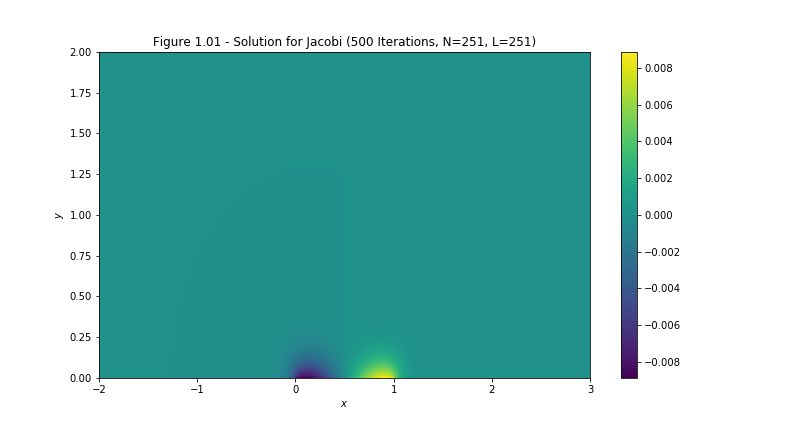
\includegraphics[width=\textwidth]{fig1.01}
    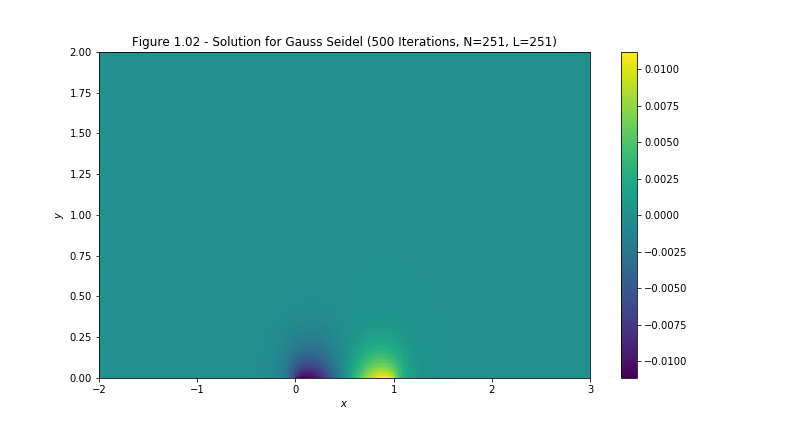
\includegraphics[width=\textwidth]{fig1.02}
    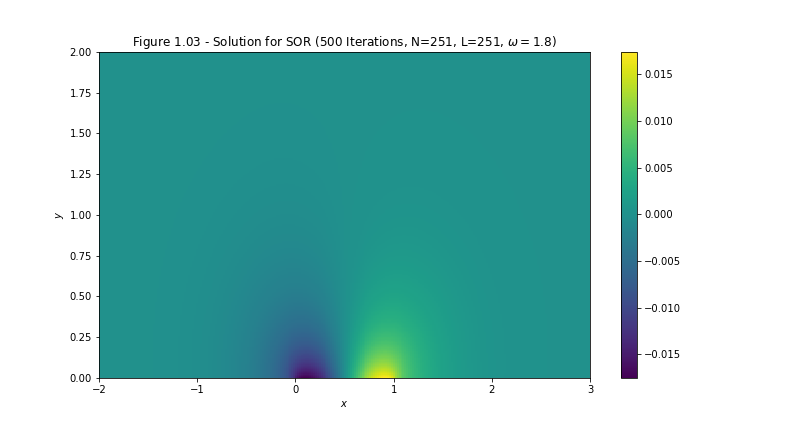
\includegraphics[width=\textwidth]{fig1.03}

    As we can see from figures 1.01, 1.02, 1.03, the solutions are very similar, however, we can see that most of our domain is still very close to zero in the Jacobi and Gauss-Seidel (GS) solutions, indicating that these methods will take much longer to converge. The SOR method contains less zero-filled region, indicating that it is further along the path of convergence, which agrees with the theory that the SOR method may be faster than both Jacobi and GS solutions. We will be exploring this behaviour in detail in the next section.

    \newpage
    \textbf{Convergence Criteria}

    For this coursework, we will be working with the relative errors from all the methods. Here, we will be working with the relative residual error between iterations defined as $error = \max|\phi^{k+1} - \phi^{k}|_{i, j}$. We can then define that a method has converged if the error value drops below a certain threshold $\theta$. The main advantage of this criteria is that it is a comparable measure of convergence accross grid sizes, thus one value of $\theta$ will suffice to define convergnece. Other norms such as the $L_1, L_2$ norms depend on the grid size.

    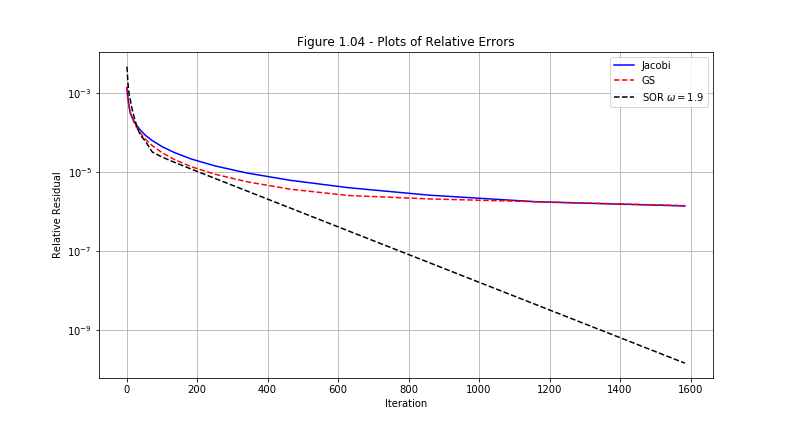
\includegraphics[width=\textwidth]{fig1.04}

    Figure 1.04 illustrates the relative residual error (define above) for all the three iterative schemes over a range of iterations. It is clear that the SOR converges to the solution very fast for large $\omega$ and we can see that the Jacobi and GS method converge much more slowly. This is to be expected, since the theory states that if the Jacobi, GS, SOR methods do converge, the Jacobi, GS converge in $\max\{O(N^2), O(L^2)\}$ iterations, whereas SOR may converge in $\max\{O(N), O(L)\}$ iterations if an optimal relaxation parameter $\omega$ exists.

    From a computational efficiency point of view, it is clear that we wish to take the iterative method that takes the least amount of computer operations. Since the three methods require roughly similar number of operations per iteration, we conclude that SOR is the clear winner here to achieve fast convergence.

    \newpage
    \textbf{Investigation of the quantities $U_{surf} (u) \text{ and } v$}

    We can find each of these quantities by taking a second-order FD approximation to the partial derivatives $u = \frac{\partial \phi}{\partial x}, v = \frac{\partial \phi}{\partial y}$. The following three figures illustrate how $u, v$  vary along the boundary $y=0$ as well as along the whole domain in Figure 1.07.

    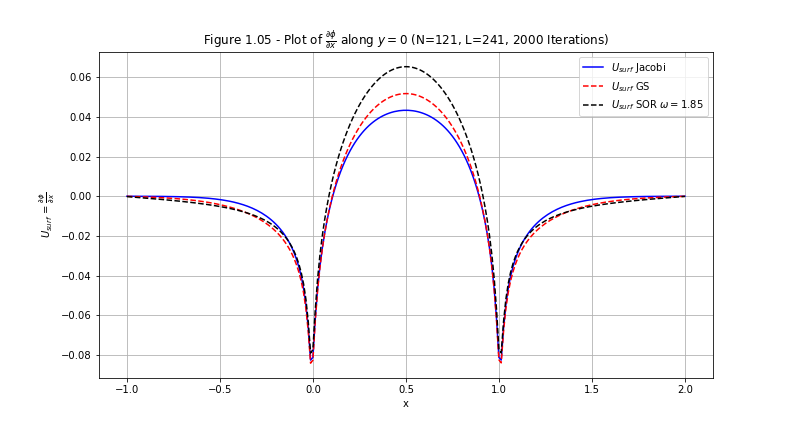
\includegraphics[width=\textwidth]{fig1.05}
    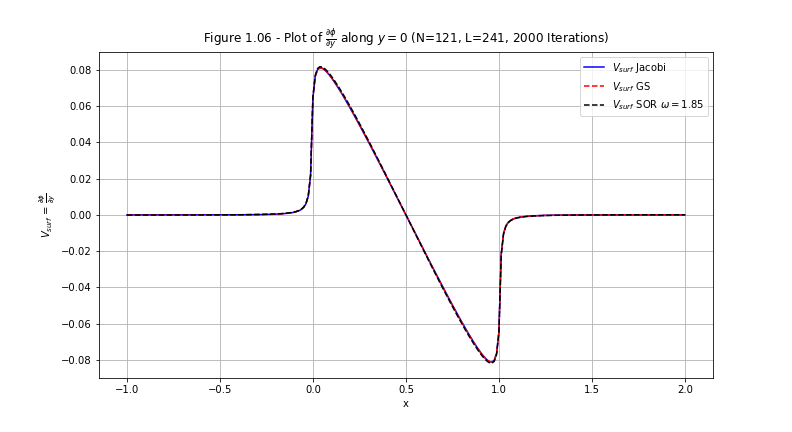
\includegraphics[width=\textwidth]{fig1.06}
    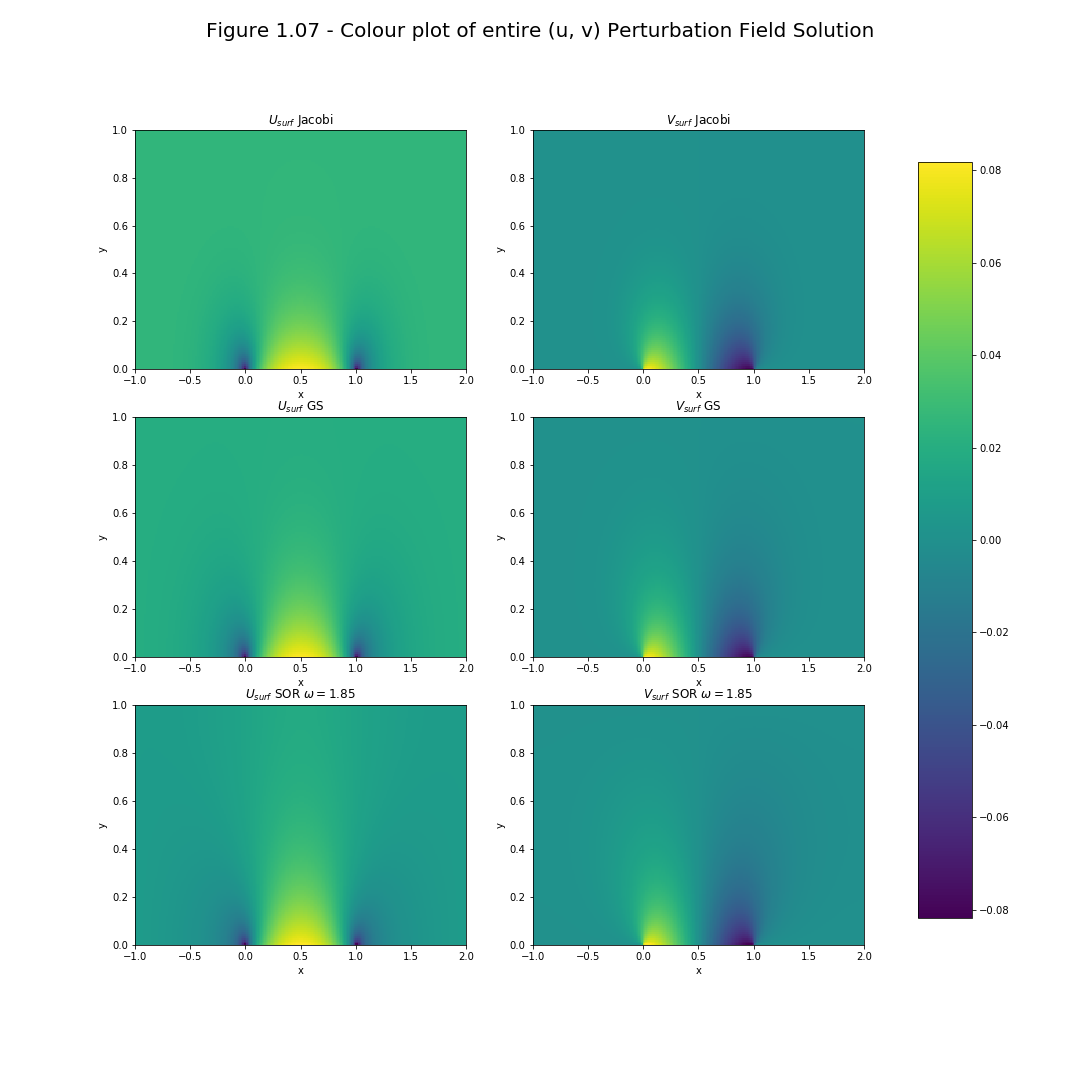
\includegraphics[width=\textwidth]{fig1.07}

    \vspace{-0.5cm}
    Figure 1.07 is a colour of the entire $(u, v)$ perturbation field solution over the complete $(x, y)$ domain, as required in the question.

    The following table contains values at the $x$-locations = (0.025, 0.25, 0.5, 0.75, 0.9) for $\tau = 0.05$ taken for $N = 121, L = 241, N_{iters}=2000.$

    \begin{center}
    \begin{tabular}{llllllll}
    \toprule
     Values & $U_{surf}$ Jacobi & $U_{surf}$ GS & $U_{surf}$ SOR & $V_{surf}$ Jacobi & $V_{surf}$ GS & $V_{surf}$ SOR\\
    \midrule
    $x = 0.025$ & -0.04698 & -0.04793 & -0.04188 & 0.08016 & 0.08014 & 0.08076 \\
    $x = 0.25$ & 0.03025 & 0.03487 & 0.04601 & 0.04964 & 0.0499 & 0.05052 \\
    $x = 0.5$ & 0.04336 & 0.05176 & 0.06534 & -0.0 & 0.0 & -0.0 \\
    $x = 0.75$ & 0.03025 & 0.03506 & 0.04607 & -0.04964 & -0.04991 & -0.05053 \\
    $x = 0.95$ & -0.00232 & -0.00143 & 0.00638 & -0.07562 & -0.07574 & -0.07644 \\
    \bottomrule
    \end{tabular}
    \end{center}

    \newpage
    \textbf{Grid Independence}

    Grid independence implies that the iterative methods converge to the same solution values independent of grid size. The convergence speed/rate depends on the coarseness of the grid, but the same solution will be reached if we let iterations tend to infinity.

    To demonstrate this, we will pick two grids, one being twice as fine as the first, and show that the $U_{surf}$ converges to similar values.

    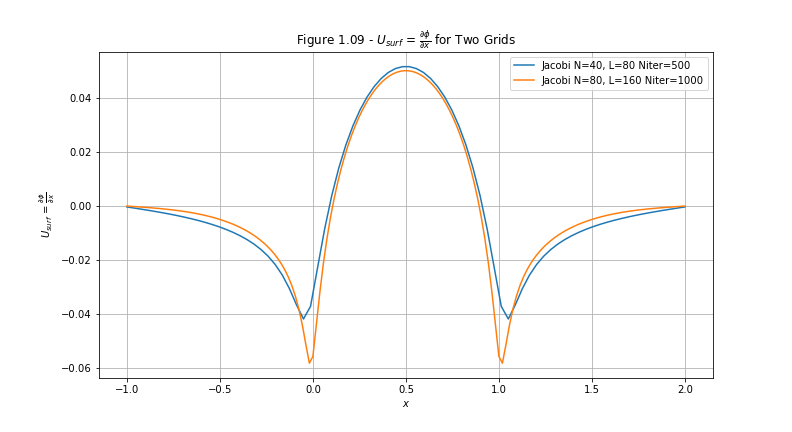
\includegraphics[width=\textwidth]{fig1.09}
    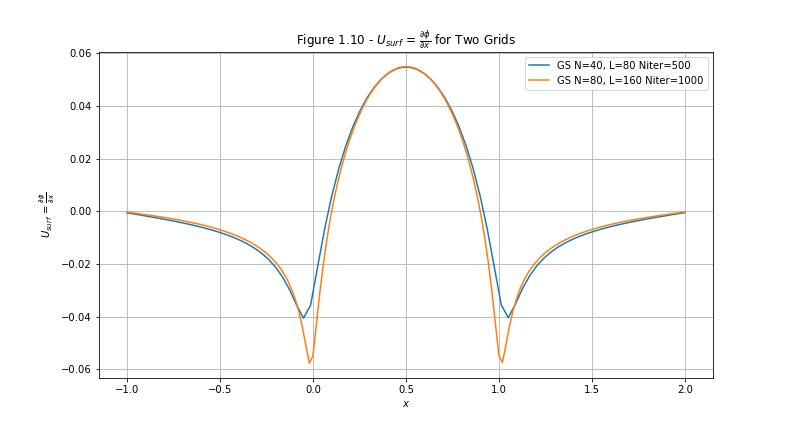
\includegraphics[width=\textwidth]{fig1.10}
    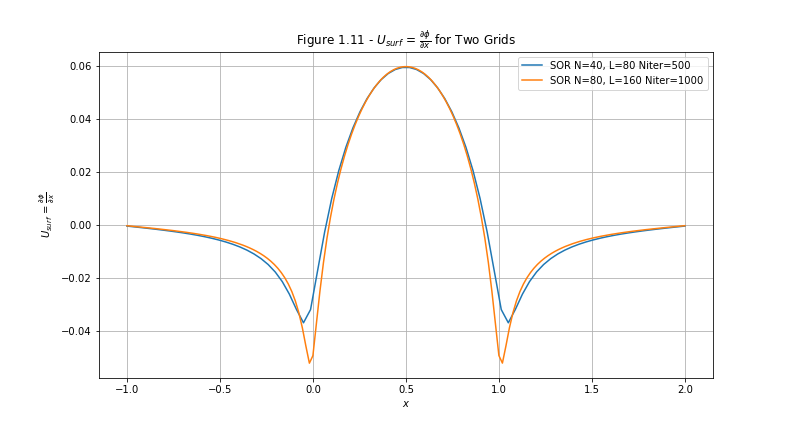
\includegraphics[width=\textwidth]{fig1.11}

    Figures 1.09, 1.10, 1.11 show that for each of the individual iterative methods, the solutions converge to the same solution, albeit at different rates.

    To deal with the far-field domain conditions, there are three ways to approach this problem. One can pick very large values of $q, s, r$ and take very large values of $N, L$, but this would be computationally very expensive. Another approach is to make $\Delta x, \Delta y$ be proportional to where we are in the plane, so we take increasingly large steps in both $x, y$ directions. In this coursework, since the 'data source' is located at $x(0:1), y=0$, we do not lose much numerical accuracy by taking $q, s, r$ relatively small.



\newpage
\section{Question 2}
    In this question, we will be working with the SOR iterative method.

    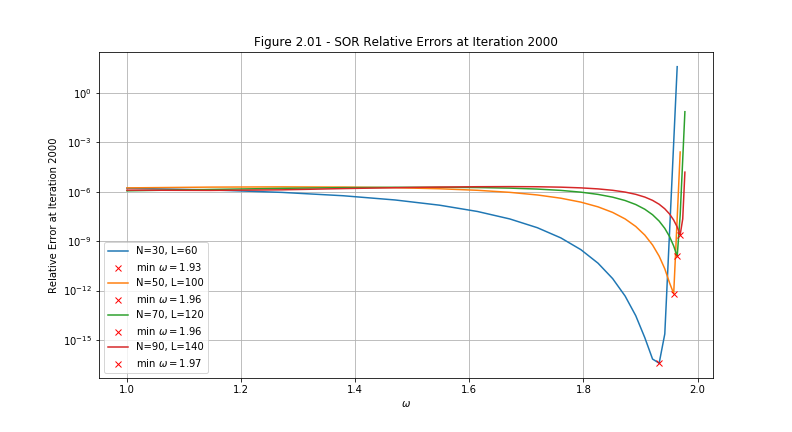
\includegraphics[width=\textwidth]{fig2.01}

    Figures 2.01 shows the final value for the relative error for SOR iterations at 2000 iterations for varying $\omega$. Each of the lines represents taking different values of $N, L$. As we can see, the optimal relaxation parameter that gives a minimum in the relative errors increases as the grid resolution increases.

    The theoretical values of optimal $\omega_{SOR}$ for the SOR method with equal grid-size is given by the formula
    \begin{equation}
        \omega_{SOR} = \frac{2}{1 + \sqrt{1 - \rho (J)^2}}, \quad \text{where} \quad \rho (J) = \cos \left(\frac{\pi}{N}\right),
    \end{equation}
    for points $i, j = 1, \ldots, N$.

    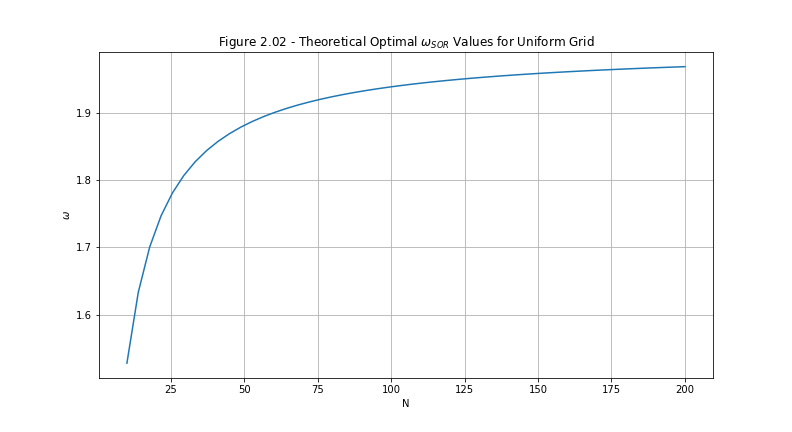
\includegraphics[width=\textwidth]{fig2.02}

    Figure 2.02 illustrates this point, and we can see that the relaxation parameter becomes very close to 2 very quickly as we increase $N$. For non-uniform grids with $L$ points in the $x$-direction and $N$ points in the $y$-direction, it can be shown that the optimal value $\omega_{SOR}$ is given by

    \begin{equation}
        \omega_{SOR} = \frac{2}{1 + \sqrt{1 - \rho (J)^2}}, \quad \text{where} \quad \rho (J) = \frac{1}{2}\left(\cos \left(\frac{\pi}{L}\right) + \cos \left(\frac{\pi}{N}\right)\right).
    \end{equation}
    If we compute these values and compare them with the optimal values attained in figure 2.01, we obtain

    \begin{center}
        \begin{tabular}{llll}
            \toprule
                Grid Size & Calculated Values & Theoretical Values \\
            \midrule
                N=30, L=50 &            1.9328 &             1.8473 \\
                N=50, L=100 &            1.9582 &             1.9054 \\
                N=70, L=120 &            1.9644 &             1.9291 \\
                N=90, L=140 &            1.9696 &              1.943 \\
            \bottomrule
        \end{tabular}
    \end{center}

    These values are close, however the discrepancy may be due to the fact that we needed to take more iterations to be closer to the theoretical values.


\newpage
\section{Question 3}
    In this question, we will be performing a coordinate transformation of the form $\eta = y - y_b(x), 0 \leq x \leq 1.$ For convenience in writing the partial derivatives, we will be doing a full-coordinate transformation from $(x, y)$ space to $(\xi, \eta)$, where we let $\xi(x, y) = x, \eta(x, y) = y - y_b(x) = y - 2\tau x(1-x)$. We can write the first partial derivatives as

    \begin{align*}
        \frac{\partial}{\partial x} &= \frac{\partial}{\partial \xi}\frac{\partial\xi}{\partial x} + \frac{\partial}{\partial \eta} \frac{\partial\eta}{\partial x} = \frac{\partial}{\partial \xi} - 2\tau(1 - 2x)\frac{\partial}{\partial \eta}, \\
        \frac{\partial}{\partial y} &= \frac{\partial}{\partial \xi}\frac{\partial\xi}{\partial y} + \frac{\partial}{\partial \eta} \frac{\partial\eta}{\partial y} = \frac{\partial\eta}{\partial y},
    \end{align*}
    and the second partial derivatives as
    \begin{align*}
        \frac{\partial^2}{\partial x^2} &= 4\tau \frac{\partial}{\partial \eta} + \frac{\partial^2}{\partial \xi^2} + 4\tau^2(1 - 2x)^2\frac{\partial^2}{\partial \eta^2} - 4\tau(1-2x)\frac{\partial^2}{\partial \xi \partial \eta}, \\
        \frac{\partial^2}{\partial y^2} &= \frac{\partial^2}{\partial \eta^2}
    \end{align*}
    Using the previous formulas, we can transform our original Laplace equation into $(\xi, \eta)$ coordinates and obtain
    \begin{equation}\label{eq:laplace_transformed}
        \frac{\partial^2\phi}{\partial \xi^2} + \frac{\partial^2\phi}{\partial \eta^2}(1 + 4\tau^2(1-2\xi)^2) + 4\tau\frac{\partial\phi}{\partial \eta} - 4\tau(1-2\xi)\frac{\partial^2\phi}{\partial \xi \partial \eta} = 0
    \end{equation}

    The inviscid flow tangency condition in $\xi, \eta$ space becomes
    \begin{equation}
        \frac{\partial\phi}{\partial \eta} - 2\tau(1-2\xi)\left(1 + \frac{\partial\phi}{\partial \xi} - 2\tau(1-2\xi)\frac{\partial\phi}{\partial \eta}\right) = 0
    \end{equation}

    \newpage
    \textbf{Discretised $(\xi, \eta)$ Laplacian}

    Using the appropriate second-order finite difference approximations to the partial derivatives w.r.t $\xi, \eta$, we can discretise the Laplacian in $\xi, \eta$ space given by equation (\ref{eq:laplace_transformed}) to obtain the following discretised equation

    \begin{align*}
        \left(\frac{2}{\Delta \xi^2} + \frac{2}{\Delta \eta^2}(1 + 4\tau^2(1-2\xi_i)^2)\right)\phi_{i,j} = \frac{\phi_{i-1, j} + \phi_{i+1, j}}{\Delta \xi^2} + \frac{\phi_{i, j+1} + \phi_{i, j-1}}{\Delta \eta^2}(1 + 4\tau^2(1-2\xi_i)^2) \\
        + 2\tau \left(\frac{\phi_{i, j+1} - \phi_{i, j-1}}{\Delta \eta}\right) - \tau(1 - 2\xi_i)\left(\frac{\phi_{i+1,j+1} - \phi_{i+1,j-1} - \phi_{i-1,j+1} + \phi_{i-1,j-1}}{\Delta \xi \Delta \eta}\right).
    \end{align*}

    This discretisation works only in the interval $\xi \in [0, 1]$. By the properties of the transformation $(x, y) \to (\xi, \eta)$, we can keep the grid uniform, we can still use the grid heights as before i.e. $(\Delta \xi, \Delta \eta)$ inside the region $x[0:1]$ equals ($\Delta x, \Delta y$) outside of the region $x(0:1)$.

    \textbf{Discretised $(\xi, \eta)$ Inviscid Fluid Condition}

    We now need to transform our inviscid fluid condition to obtain the following equation used to solve for the fictitious points below the boundary of the airfoil:
    \begin{equation}
        \phi_{i, 0} = \phi_{i, 2} - \frac{4\tau\Delta \eta (1 - 2\xi_i)}{(1 + 4\tau^2(1 - 2\xi_i)^2)} -  \frac{2\Delta \eta \tau(1-2\xi_i)}{\Delta \xi (1 + 4\tau^2(1 - 2\xi_i)^2)}(\phi_{i+1, 1} - \phi_{i-1, 1}).
    \end{equation}

    Using these two equations, we can iterate using SOR similarly to before, only that in the region $x(0:1)$ we take care to use the transformed version of our equations instead.

    Numerically, this scheme is much more complicated than the scheme studied in Q1, and we can see a dependence of $\xi_i (=x_i)$ inside the SOR iteration, so we will need to keep track of the values of $\xi_i (=x_i) $ when iterating through our domain.

    Another challenging numerical feature of this transformation is that it introduces a discontinuity (a stagnation point) in our domain at $\xi=0$ and at $\xi=1$. To capture the full behaviour of the solution at these points, we will need to grid points very close in those regions. This can be done by making the full grid much more fine, or by making $\Delta \xi$ vary in our domain, taking smaller values around these points and letting $\Delta \xi$ become larger as we move away from these regions.

    \newpage
    \textbf{Verification of Implementation and Comparison with Q1}

    We can plot the result of this discretisation with the one in Q1 by plotting $U_{surf}$ and $V_{surf}$ for both discretisations keeping the same other parameters:

    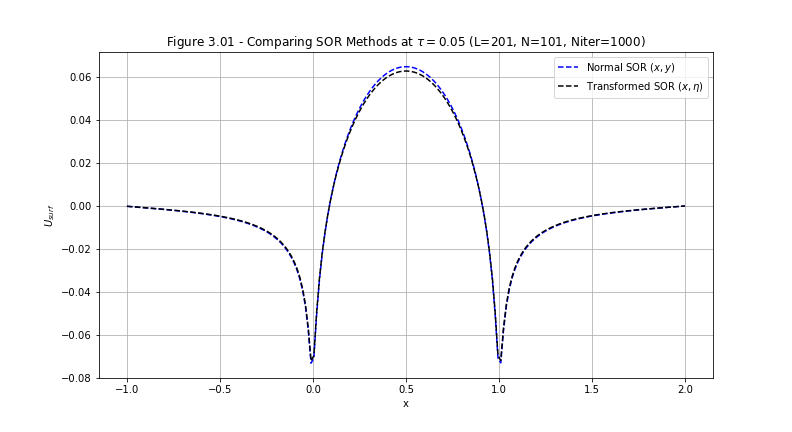
\includegraphics[width=\textwidth]{fig3.01}
    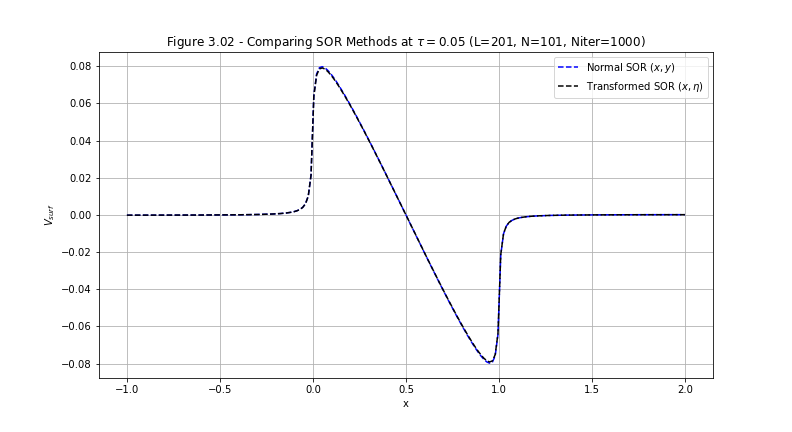
\includegraphics[width=\textwidth]{fig3.02}

    Figures 3.01 and 3.02 clearly shows that the results are very similar indeed for small $\tau=0.05$, showing that transferring the boundary to $y=0$ is indeed a good approximation for small $\tau$.

    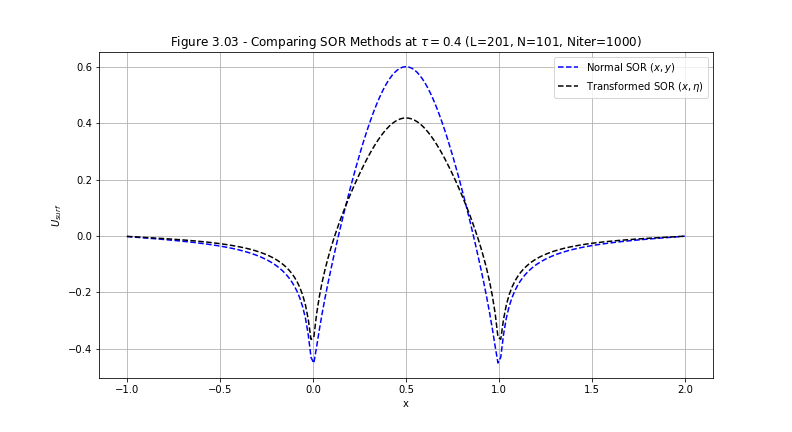
\includegraphics[width=\textwidth]{fig3.03}
    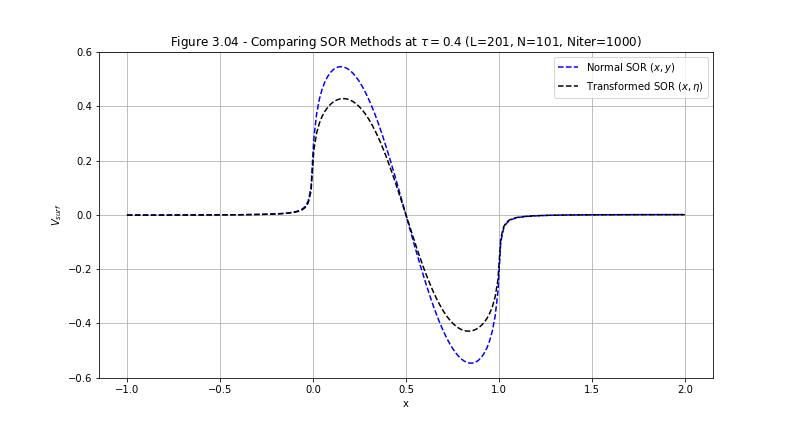
\includegraphics[width=\textwidth]{fig3.04}

    Figures 3.03 and 3.04 show the differences in $U_{surf}$ and $V_{surf}$ for a much larger $\tau = 0.4$. As we can see, the solutions differ now, indicating that the approximation used in Q1 becomes less accurate as we increase $\tau$.

    In the following plot, we will be investigating how much $U_{surf}$ and $V_{surf}$ change for both discretisations. To do this, we will be varying $\tau$ between 0.001 and 0.4  while keeping all other parameters the same and compute the difference in solutions as $||U_{surf}^{SOR_1}  - U_{surf}^{SOR_2}||_2$ and $||V_{surf}^{SOR_1}  - V_{surf}^{SOR_2}||_2$:

    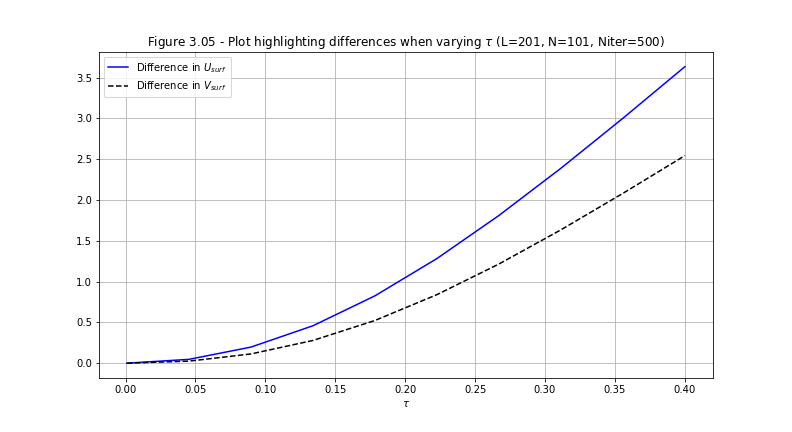
\includegraphics[width=\textwidth]{fig3.05}

    Figure 3.05 clearly shows that the differences increase as we take higher $\tau$, which is to be expected, since the boundary $y_b(x)$ is a quadratic with leading coefficient $-2\tau$, hence we expect the approximation of transfering $y_b(x)$ to $y=0$ to get worse and worse (quadratically) as we increase $\tau$.


\newpage
\section{Question 4}

    In this question we will be developing a multigrid approach to solving the Poisson equation. The motivation behind multigrid is that the Gauss-Seidel (GS) iteration is poor at resolving low frequency errors when taking a grid that is fine enough to achieve desired $O(h^2 + k^2)$ accuracy. We can apply the GS on a coarser grid to get rid of the low-frequency errors, however, in that coarse grid, we will not be able to resolve the high-frequency errors. Hence, the multigrid tackles this idea by performing GS on grids of different levels of coarseness.

    The file \texttt{multigrid.py}, contains the class \texttt{MultiGrid} which contains code to perform V-cycles for multigrid. In the 2-grid approach, one V-Cycle goes as follows:

    \textbf{V-Cycle}
    \begin{enumerate}
        \item Compute the residual, refined as $r = f - \mathscr{L}\phi_1$, where $\mathscr{L}$ denotes solving our Laplacian equation.
        \item Do $n$ iterations of GS on the finest grid, for some number of iterations $n$, starting from an initial guess $\phi$, to obtain an estimate $\phi_1$.
        \item \textbf{Restrict} the residual to the coarsest grid of, say, twice the coarseness.
        \item Do $m$ iterations of GS on the coarser grid, for some number of iterations $m$, to obtain a coarser version of our solution $\phi_2$.
        \item \textbf{Interpolate} the residual back to the finest grid and add this error to $\phi_1$ to obtain $\phi_3$.
        \item Do $l$ final iterations of GS on the finest starting from $\phi_3$.
    \end{enumerate}

    We can choose to use more grids than just two, as well as perform multiple V-Cycles to achieve the desired accuracy or performance to our problem.

    It remains to define what the restrict and interpolate operations mean. In our implementation, the restriction operation consists of taking a weighted average of the nearest neighbours on our finer grid. We are free to choose what this weighted average is, and in fact it turns out that we can make our restriction more or less accurate (and efficient) depending on how many neighbours we wish to take into account for each point in the fine grid.

    The interpolation operation is more complicated, but in our implementation, it is the one given in the lectures (Lecture 12-13 Introduction to Multigrid).

    In the implementation, the class \texttt{MultiGrid} contains vectorised methods of interpolate, restrict and residual, as well as helper methods for calculating the boundary conditions used  in the GS iteration.

    The class is flexible enough to add different multigrid routines, such as F or W cycles.

    \newpage
    \textbf{Verification of Implementation}

    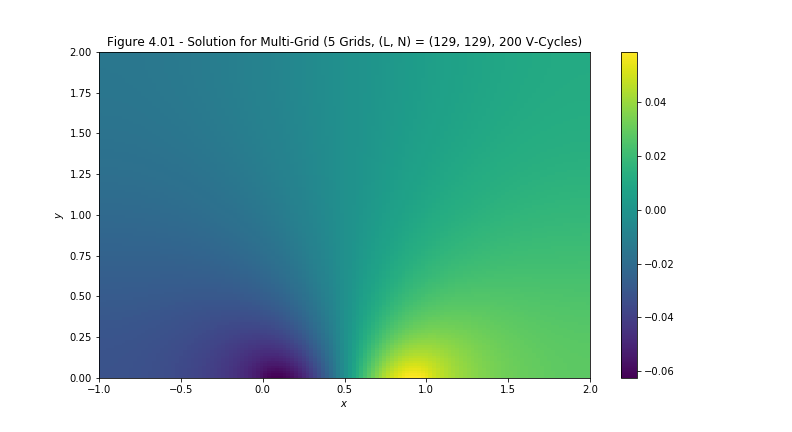
\includegraphics[width=\textwidth]{fig4.01}
    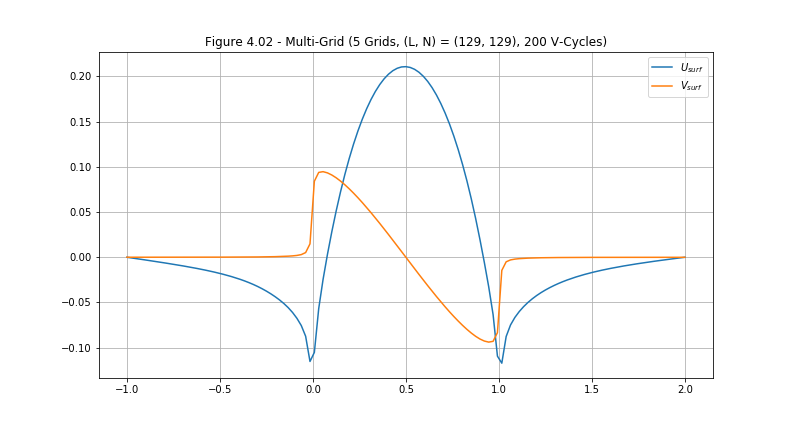
\includegraphics[width=\textwidth]{fig4.02}

    Figures 4.01, 4.02 shows the output of the Multi-Grid algorithm after 200 V-Cycles, using 10 GS iterations for each smoothing operation at each grid.

    \newpage
    \textbf{Investigation of Convergence Properties}

    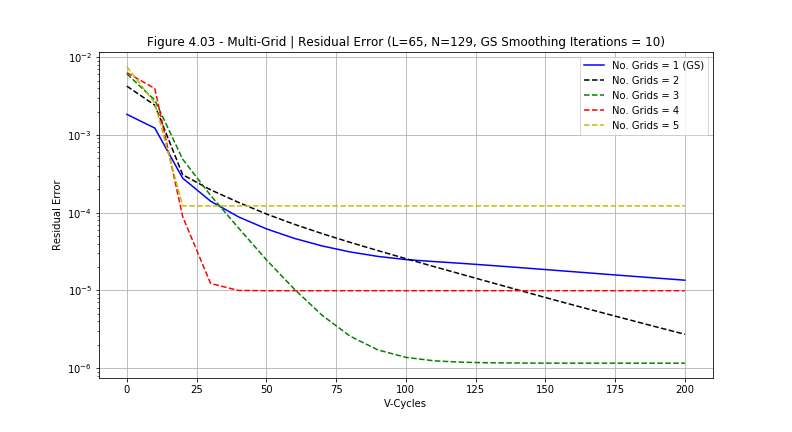
\includegraphics[width=\textwidth]{fig4.03}

    Figure 4.03 shows how the residual error evolves with V-Cycle iterations for the grid size $N=65, L=129$ changing the number of grids that we use. Using 1 grid is the same as doing GS iteration so we will use the blue line as reference for comparison with Q1. As we can see, we achieve the lowest accuracy $(\approx 10^{-6})$ when using 3 grids. This corresponds to the coarsest grid being $N=17, L=33$. Going any further than 4 grids does not improve accuracy in this case. If a residual error of $(\approx 10^{-6})$ is needed, then using 3 grids is superior in terms of computer timing than simple GS, since the number of iterations is far lower to achieve this level of convergence, and as we know from lectures, GS iterations at the coarser grids are far less expensive than taking many times more GS iterations to achieve the same level of accuracy.

    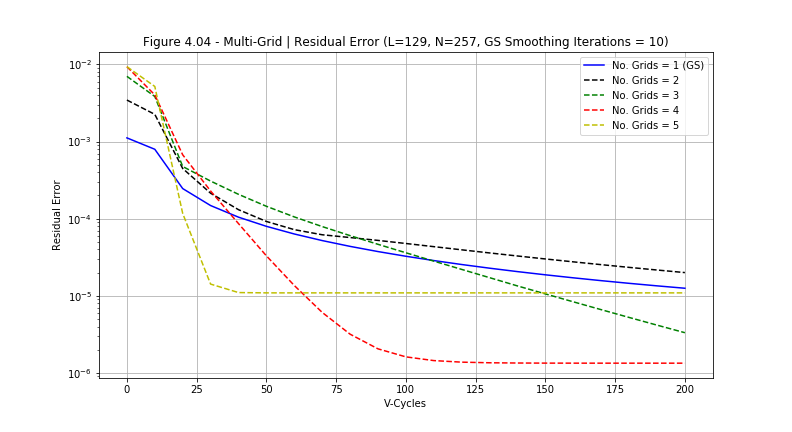
\includegraphics[width=\textwidth]{fig4.04}

    Figure 4.04 shows how the residual error evolves with V-Cycle iterations with a grid that is twice as fine as the grid used to produce Figure 4.03, i.e. $N=129, L=257$. This time, we see that taking 4 grids gives the best $(\approx 10^{-6})$ residual error. The coarsest grid is again taking  $N=17, L=33$, hence we can deduce that if we want to minimise residual error as quickly as possible to the $(\approx 10^{-6})$, we should make a general multigrid use this grid ($N=17, L=33$) as it's coarsest level.

    If we want to achieve higher precision, we may be forced to choose a finer grid as our coarsest grid, as can be seen by the line No. Grids = 3 which may drop in residual error further for larger iterations and so further iterations may be needed if lower residual error is needed for a particular reason.

    We can conclude that the multigrid approach does improve our iteration speed when compared with simple Gauss-Seidel and therefore lowes computational cost and time needed to solve this numerical problem.

    \textbf{Remark}: To achieve better accuracy still, we could introduce the transformation used in Q3. To do this, we would need to modify our boundary conditions, change the Gauss-Seidel iteration and modify our residual routines. Otherwise, the restrict, interpolate and v-cycle routines would stay unchanged.

\end{document}
